\chapter{	结构体、文字显示与GDT/IDT初始化	}
\section{	接收启动信息(harib02a)	}
在bootpack.c里面中直接将0xa0000、320、200这种数字直接写入程序,而本来这些值应该从asmhead.nas先前保存下来的值中取。如果不这样,当画面模式改变时,系统就不能正常运行。

使用指针来取得这些值。

\dag|projects\05_day\harib02a|
\begin{code}[label=bootpack.c 节选]
void HariMain(void)
{
	char *vram;
	int xsize, ysize;
	short *binfo_scrnx, *binfo_scrny;
	int *binfo_vram;

	init_palette();
	binfo_scrnx = (short *) 0x0ff4;
	binfo_scrny = (short *) 0x0ff6;
	binfo_vram = (int *) 0x0ff8;
	xsize = *binfo_scrnx;
	ysize = *binfo_scrny;
	vram = (char *) *binfo_vram;
\end{code}

这里的0x0ff4之类的地址仅仅是为了与asmhead.nas保持一致才出现的。

另外,把显示画面背景的部分独立出来,单独做成一个函数init\_screen。
\section{	试用结构体(harib02b)	}
使用结构体的方式重写主程序。
\dag|projects\05_day\harib02b|
\begin{code}[label=bootpack.c 节选]
struct BOOTINFO {
	char cyls, leds, vmode, reserve;
	short scrnx, scrny;
	char *vram;
};

void HariMain(void)
{
	char *vram;
	int xsize, ysize;
	struct BOOTINFO *binfo;

	init_palette();
	binfo = (struct BOOTINFO *) 0x0ff0;
	xsize = (*binfo).scrnx;
	ysize = (*binfo).scrny;
	vram = (*binfo).vram;
\end{code}
\section{	试用箭头记号(harib02c)	}
C语言中常常会用到类似于(*binfo).scrnx的表现手法,因此出现了一种不使用括号的省略表现方式,即binfo->scrnx,称之为箭头标记方式。
\dag|projects\05_day\harib02c|
\begin{code}[label=bootpack.c 节选]
void HariMain(void)
{
	struct BOOTINFO *binfo = (struct BOOTINFO *) 0x0ff0;

	init_palette();
	init_screen(binfo->vram, binfo->scrnx, binfo->scrny);
\end{code}
上面几小节都是C语言的写法问题,编译成机器语言以后几乎没什么差别。只是后面的这些写法更简洁清晰一些。
\section{	显示字符(harib02d)	}
使用8$\times$16的长方形像素点阵来表示字符。

%\begin{figure}[H]
%  \centering
%  % Requires \usepackage{graphicx}
%  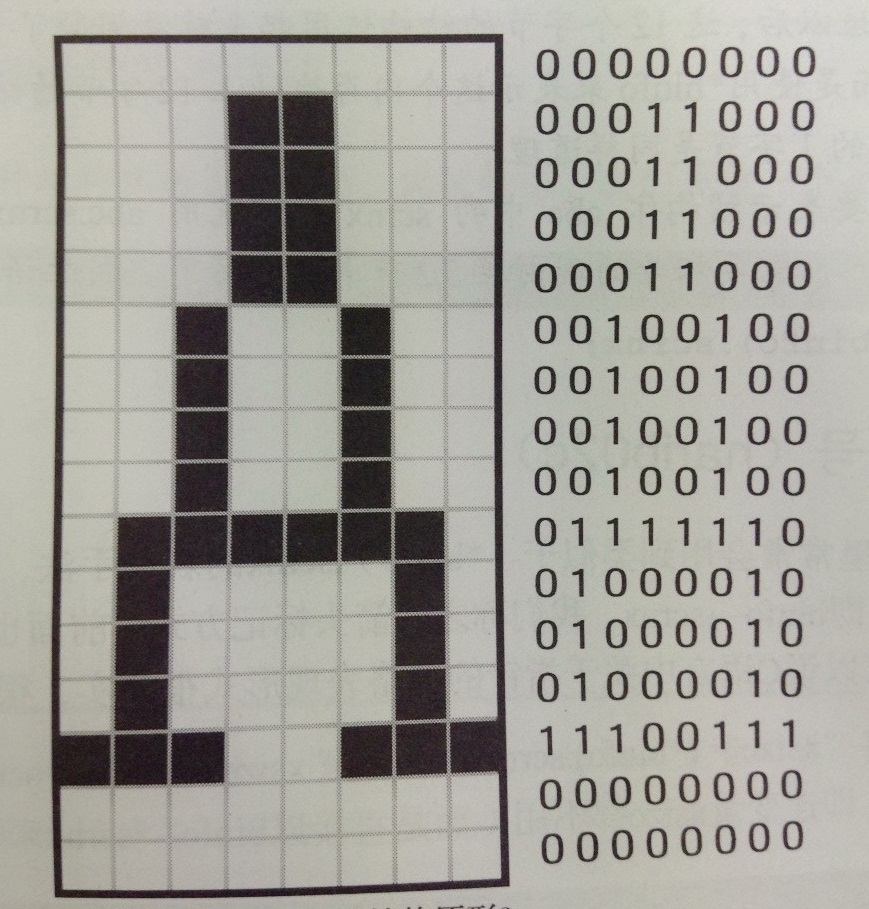
\includegraphics[height=0.4\textheight]{day05-zifua.jpg}\\
%\end{figure}

像这种描述文字形状的数据称为字体数据,通过数组来保存,写入程序。
\dag|projects\05_day\harib02d|
\begin{code}[label=bootpack.c节选]
\begin{code}
	static char font_A[16] = {
		0x00, 0x18, 0x18, 0x18, 0x18, 0x24, 0x24, 0x24,
		0x24, 0x7e, 0x42, 0x42, 0x42, 0xe7, 0x00, 0x00
	};
\end{code}
用for语句将画8个像素的程序循环16遍,就可以显示出一个字符了。
\begin{code}[label=bootpack.c节选]
void putfont8(char *vram, int xsize, int x, int y, char c, char *font)
{
	int i;
	char *p, d /* data */;
	for (i = 0; i < 16; i++) {
		p = vram + (y + i) * xsize + x;
		d = font[i];
		if ((d & 0x80) != 0) { p[0] = c; }
		if ((d & 0x40) != 0) { p[1] = c; }
		if ((d & 0x20) != 0) { p[2] = c; }
		if ((d & 0x10) != 0) { p[3] = c; }
		if ((d & 0x08) != 0) { p[4] = c; }
		if ((d & 0x04) != 0) { p[5] = c; }
		if ((d & 0x02) != 0) { p[6] = c; }
		if ((d & 0x01) != 0) { p[7] = c; }
	}
	return;
}
\end{code}

运行“make run”,可以显示大写字符“A”出来。
\section{	增加字体(harib02e)	}
使用已经做好的字体库hankaku.txt(程序目录下有)。
\cs

由于字库仅是简单的字符,需要专用的“编译器”来使字库可以被程序调用。

makefont.exe将上面的文本文件(256个字符的字体文件)读进来,然后输出成16$\times$256=4096字节的hankaku.bin文件。使用bin2obj.exe加上链接所必要的接口信息,将它变成目标文件。

如果在C语言中使用这种字体数据,只需要写上以下语句就可以了。

|extern char hankaku[4096];|

像这种在源程序以外准备的数据,都需要加上extern属性。

\cs

OSAKA的字体数据,依照一般的ASCII字符编码,含有256个字符。A的字符编码是0x41,所以A的字体数据放在在“|hankaku+0x41*16|”开始的16个字节里。C语言中的字符编码可以用‘A’来表示,即可以写成“|hankaku+'A'*16|”。

程序添加了“ABC 123”,运行以下试试看。

\dag|projects\05_day\harib02e|
\begin{code}[label=bootpack.c]
void HariMain(void)
{
	struct BOOTINFO *binfo = (struct BOOTINFO *) 0x0ff0;
	extern char hankaku[4096];

	init_palette();
	init_screen(binfo->vram, binfo->scrnx, binfo->scrny);
	putfont8(binfo->vram, binfo->scrnx,  8, 8, COL8_FFFFFF, hankaku + 'A' * 16);
	putfont8(binfo->vram, binfo->scrnx, 16, 8, COL8_FFFFFF, hankaku + 'B' * 16);
	putfont8(binfo->vram, binfo->scrnx, 24, 8, COL8_FFFFFF, hankaku + 'C' * 16);
	putfont8(binfo->vram, binfo->scrnx, 40, 8, COL8_FFFFFF, hankaku + '1' * 16);
	putfont8(binfo->vram, binfo->scrnx, 48, 8, COL8_FFFFFF, hankaku + '2' * 16);
	putfont8(binfo->vram, binfo->scrnx, 56, 8, COL8_FFFFFF, hankaku + '3' * 16);

	for (;;) {
		io_hlt();
	}
}
\end{code}
\section{	显示字符串(harib02f)	}
可以直接显示字符串,而不是一个个字符写在程序里。

\dag|projects\05_day\harib02f|
\begin{code}[label=bootpack.c]
void putfonts8_asc(char *vram, int xsize, int x, int y, char c, unsigned char *s)
{
	extern char hankaku[4096];
	for (; *s != 0x00; s++) {
		putfont8(vram, xsize, x, y, c, hankaku + *s * 16);
		x += 8;
	}
	return;
}
\end{code}

使用显示字符串的方法来炫一下。
\begin{code}[label=bootpack.c]
void HariMain(void)
{
	struct BOOTINFO *binfo = (struct BOOTINFO *) 0x0ff0;

	init_palette();
	init_screen(binfo->vram, binfo->scrnx, binfo->scrny);
	putfonts8_asc(binfo->vram, binfo->scrnx,  8,  8, COL8_FFFFFF, "ABC 123");
	putfonts8_asc(binfo->vram, binfo->scrnx, 31, 31, COL8_000000, "Haribote OS.");
	putfonts8_asc(binfo->vram, binfo->scrnx, 30, 30, COL8_FFFFFF, "Haribote OS.");

	for (;;) {
		io_hlt();
	}
}
\end{code}
\section{	显示变量值(harib02g)	}
显示变量的值,这个很有用,因为这里没有调试器,调试系统不是很容易,所以还是打印变量值来看看到底哪里不对了。由于在自制操作系统中不能随便使用printf函数,但可以使用sprintf,它不是按制定格式输出,只是将输出的内容作为字符串写在内存中,所以可以应用于所有操作系统。

这里用的sprintf函数是本次使用的名为GO的C编译器附带的函数。

\cs

添加头文件|#include<stdio.h>|。

sprintf函数的使用方法是:sprintf(地址,格式,值,值,值,$\cdots\cdots$)。其中,格式和C语言中的定义一样,\verb|%d,%x|这种。
\begin{code}
    sprintf(s, "scrnx = %d", binfo->scrnx);
	putfonts8_asc(binfo->vram, binfo->scrnx, 16, 64, COL8_FFFFFF, s);
\end{code}
\section{	显示鼠标指针(harib02h)	}
将鼠标指针的大小定为16$\times$16。

\dag|projects\05_day\harib02h|
\begin{code}[label=bootpack.c]
void init_mouse_cursor8(char *mouse, char bc)
/* マウスカーソルを準備(16x16) */
{
	static char cursor[16][16] = {
		"**************..",
		"*OOOOOOOOOOO*...",
		"*OOOOOOOOOO*....",
		"*OOOOOOOOO*.....",
		"*OOOOOOOO*......",
		"*OOOOOOO*.......",
		"*OOOOOOO*.......",
		"*OOOOOOOO*......",
		"*OOOO**OOO*.....",
		"*OOO*..*OOO*....",
		"*OO*....*OOO*...",
		"*O*......*OOO*..",
		"**........*OOO*.",
		"*..........*OOO*",
		"............*OO*",
		".............***"
	};
	int x, y;

	for (y = 0; y < 16; y++) {
		for (x = 0; x < 16; x++) {
			if (cursor[y][x] == '*') {
				mouse[y * 16 + x] = COL8_000000;
			}
			if (cursor[y][x] == 'O') {
				mouse[y * 16 + x] = COL8_FFFFFF;
			}
			if (cursor[y][x] == '.') {
				mouse[y * 16 + x] = bc;
			}
		}
	}
	return;
}
\end{code}
变量bc是指back-color,也就是背景色。

要将背景色显示出来,只要将buf中的数据复制到vram中去就可以了。
\begin{code}[label=bootpack.c]
void putblock8_8(char *vram, int vxsize, int pxsize,
	int pysize, int px0, int py0, char *buf, int bxsize)
{
	int x, y;
	for (y = 0; y < pysize; y++) {
		for (x = 0; x < pxsize; x++) {
			vram[(py0 + y) * vxsize + (px0 + x)] = buf[y * bxsize + x];
		}
	}
	return;
}
\end{code}
函数中,vram和vxsize是关于VRAM的信息,值分别为0xa0000和320。pxsize和pysize是想要显示的图形的大小,这里是鼠标指针的大小16。px0和py0指定图形在画面上的显示位置。最后的buf和bxsize分别指定图形的存放地址和每一行含有的像素数。

调用函数:
\begin{code}[label=bootpack.c]
    init_mouse_cursor8(mcursor, COL8_008484);
	putblock8_8(binfo->vram, binfo->scrnx, 16, 16, mx, my, mcursor, 16);
\end{code}

\section{	GDT与IDT的初始化(harib02i)	}

上节中,鼠标显示出来了,但是无法移动。需要通过初始化GDT和IDT来完成移动。

GTD(global (segment) descriptor table),全局段号记录表。将这些数据整齐的排列在内存的某个地方,然后将内存的起始地址和有效设定个数放在CPU内被称为GDTR的特殊寄存器中,设定就完成了。

IDT(interrupt descriptor table),中断记录表。IDT记录了0$\sim$255号中段号码与调用函数的对应关系。

\dag|projects\05_day\harib02i|
\begin{code}[label=bootpack.c节选]
struct SEGMENT_DESCRIPTOR {
	short limit_low, base_low;
	char base_mid, access_right;
	char limit_high, base_high;
};

struct GATE_DESCRIPTOR {
	short offset_low, selector;
	char dw_count, access_right;
	short offset_high;
};

void init_gdtidt(void)
{
	struct SEGMENT_DESCRIPTOR *gdt = (struct SEGMENT_DESCRIPTOR *) 0x00270000;
	struct GATE_DESCRIPTOR    *idt = (struct GATE_DESCRIPTOR    *) 0x0026f800;
	int i;

	/* GDTの初期化 */
	for (i = 0; i < 8192; i++) {
		set_segmdesc(gdt + i, 0, 0, 0);
	}
	set_segmdesc(gdt + 1, 0xffffffff, 0x00000000, 0x4092);
	set_segmdesc(gdt + 2, 0x0007ffff, 0x00280000, 0x409a);
	load_gdtr(0xffff, 0x00270000);

	/* IDTの初期化 */
	for (i = 0; i < 256; i++) {
		set_gatedesc(idt + i, 0, 0, 0);
	}
	load_idtr(0x7ff, 0x0026f800);

	return;
}

void set_segmdesc(struct SEGMENT_DESCRIPTOR *sd, unsigned int limit, int base, int ar)
{
	if (limit > 0xfffff) {
		ar |= 0x8000; /* G_bit = 1 */
		limit /= 0x1000;
	}
	sd->limit_low    = limit & 0xffff;
	sd->base_low     = base & 0xffff;
	sd->base_mid     = (base >> 16) & 0xff;
	sd->access_right = ar & 0xff;
	sd->limit_high   = ((limit >> 16) & 0x0f) | ((ar >> 8) & 0xf0);
	sd->base_high    = (base >> 24) & 0xff;
	return;
}

void set_gatedesc(struct GATE_DESCRIPTOR *gd, int offset, int selector, int ar)
{
	gd->offset_low   = offset & 0xffff;
	gd->selector     = selector;
	gd->dw_count     = (ar >> 8) & 0xff;
	gd->access_right = ar & 0xff;
	gd->offset_high  = (offset >> 16) & 0xffff;
	return;
}
\end{code}

SEGMENT\_DESCRIPTOR中存放GDT的8字节的内容,GATE\_DESCRIPTOR中存放IDT的8字节内容。

变量gdt被赋值为0x00270000,也就是将0x270000$\sim$0x27ffff设为GDT(从内存分布图可以看到这一块地方没有被使用)。

变量idt被设为0x26f800$\sim$0x26ffff。
\cs

\begin{code}
for (i = 0; i < 8192; i++) {
		set_segmdesc(gdt + i, 0, 0, 0);
	}
\end{code}

for循环完成对8192个段的设定,将它们的上限(limit,指段的字节数-1),基址、访问权限都设置为0。

\begin{code}
    set_segmdesc(gdt + 1, 0xffffffff, 0x00000000, 0x4092);
	set_segmdesc(gdt + 2, 0x0007ffff, 0x00280000, 0x409a);
\end{code}

以上语句对段号为1和2的两个段进行设定。段号为1的段,上限值为0xffffffff即大小正好为4GB,地址是0,它表示的是CPU所能管理的全部内存本身。段属性设置为0x4092。段号为2的段,它的大小是512KB,地址是0x280000,这正好是为bootpack.hrb准备的,用这个段,就可以执行bootpack.hrb,因为bootpack.hrb是以ORG~0为前提翻译成机器语言的。

\begin{code}
  load_gdtr(0xffff, 0x00270000);
\end{code}

因为C语言不能给GDTR赋值,借助汇编语言来赋值。

后面关于IDT的描述跟前面一样。

后面的set\_segmdesc和set\_gatedesc函数中用到了一些新的运算符,“\verb"|"”、“/”、“>>” 等,自己看吧。